Das \eigenname{QPI-SQL} Projekt hatte zum Ziel ein Fragenplugin für \eigenname{ILIAS} zu entwickeln, mit dem das \eigenname{SQL} Wissen von Testteilnehmern abgeprüft werden kann. Dieses Plugin trägt, nach den Namensschema, dass \eigenname{ILIAS} vorgibt, den Namen \eigenname{assSQLQuestion}. 
Während dieses Kapitel nicht den Umfang hat, um jedes Detail der internen Struktur von \eigenname{assSQLQuestion} näher zu erläutern, konzentriert es sich auf die dort zu findenden Besonderheiten. Dabei wird auf der einen Seite erläutert, wie der \eigenname{Javascript} Code aufgebaut ist (s. Kapitel \ref{sec:javascript}). Auf der anderen Seite wird die Besonderheit der GUI Klassen von \eigenname{assSQLQuestion} näher aufgeschlüsselt (s. Kapitel \ref{sec:gui-klassen}).

\section{Javascript}
\label{sec:javascript}

Die Struktur des \eigenname{Javascript} Codes in \eigenname{assSQLQuestion} ist dahingehend besonders, dass zum einen nicht alle \eigenname{ILIAS} Fragenplugins \eigenname{Javascript} für ihre Zwecke nutzen - siehe beispielsweise \eigenname{assExampleQuestion}. Aber auch weil der \eigenname{Javascript} Code, bei dem aus dem \eigenname{QPI-SQL} Projekt entstandenen Plugin, besondere Aufgaben zu erfüllen hat. Daraus resultieren auch besondere Klassen.

Auf der einen Seite stehen hier die sogenannten \eigenname{ExecutionInputs} und \eigenname{ExecutionOutputs}. Dies sind Javascript Klassen, die implementiert wurden, um das Einlesen von Daten aus \eigenname{HTML} Elementen (\eigenname{ExecutionInputs}), so wie die Ausgabe in selbige (\eigenname{ExecutionOutputs}), von der eigentlichen Javascript Logik zu trennen.

In Abbildung \ref{fig:execution-inputs} ist eine Übersicht über die \eigenname{ExecutionInputs} zu sehen. Mit Hilfe von \eigenname{HiddenFieldInput} können Inhalte aus versteckten Feldern ausgelesen werden, während \eigenname{HiddenTextareaInput} die selbe Aufgabe für unsichtbare Textbereiche übernimmt. Der aktuelle Wert des Kontrollkästchens zum Setzten eines Integritätschecks kann mit \eigenname{IntegrityCheckCheckboxInput} ausgelesen werden, während die wichtigste Eingabe - die Eingabe von \eigenname{SQL} Sequenzen - über \eigenname{SequenceTextareaInput} abgerufen werden kann.

    \begin{figure}[H]
        \begin{center}
            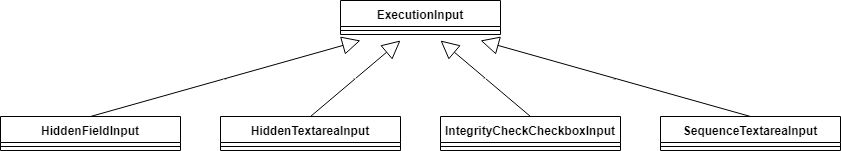
\includegraphics[page=1, width=0.7\paperwidth, trim=0 0 0 0, clip]{fig/ExecutionInputs.png} 
            \caption{Übersicht über die ExecutionInputs}
            \label{fig:execution-inputs}
        \end{center}
    \end{figure}
    
Eine ähnliche Struktur haben die \eigenname{ExecutionOutputs} (s. Abbildung \ref{fig:execution-outputs}) - die Klassen die für die Ausgabe in \eigenname{HTML} zuständig sind. \eigenname{OutputAreaOutput} ist dabei dafür zuständig die Ergebnisse von \eigenname{SQL} Durchläufen auf der Seite anzuzeigen, während \eigenname{ScoringMetricEditQuestion} und \eigenname{ScoringMetricOutputQuestion} die Ausgabe der Bewertungsmetriken übernehmen.

Hierbei ist zu beachten, dass die Ausgabe, die die \eigenname{ExecutionOutputs} kapseln sollen, auch dazu dient, Eingabefelder zu aktivieren beziehungsweise zu deaktivieren. So können mit Hilfe von \eigenname{ExecuteButtonOutput}, \eigenname{IntegrityCheckCheckboxOutput} und \eigenname{SequenceTextareaOutput} die entsprechenden Eingabeelemente deaktiviert und aktiviert werden.
    
    \begin{figure}[H]
        \begin{center}
            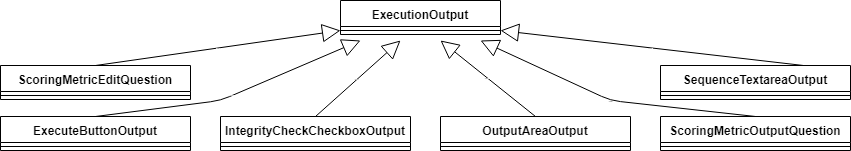
\includegraphics[page=1, width=0.7\paperwidth, trim=0 0 0 0, clip]{fig/ExecutionOutputs.png} 
            \caption{Übersicht über die ExecutionOutputs}
            \label{fig:execution-outputs}
        \end{center}
    \end{figure}

Anders als die \eigenname{ExecutionInputs} und \eigenname{ExecutionOutputs} sind einige Klassen von \eigenname{assSQLQuestion} für die Logik im \eigenname{Javascript} Code zuständig. Diese Klassen managen die gesamte Ausführung von \eigenname{SQL}. Die Klasse \eigenname{SQLRun} (s. Abbildung \ref{fig:sql-run}) steht für einen einzelnen Durchlauf von \eigenname{SQL}-Sequenzen. Dabei übergibt \eigenname{SQLRun} die Sequenzen an einen \eigenname{SQL.js} Worker-Thread und verwaltet auch einen eventuellen Integritätscheck.

    \begin{figure}[H]
        \begin{center}
            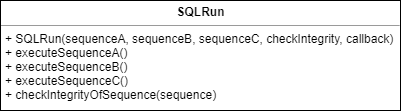
\includegraphics[page=1, width=0.5\paperwidth, trim=0 0 0 0, clip]{fig/SQLRun.png} 
            \caption{Die Methoden der Klasse SQLRun}
            \label{fig:sql-run}
        \end{center}
    \end{figure}

Die Klasse \eigenname{SQLResult} ist dagegen das Ergebniss, dass ein erfolgreicher \eigenname{SQLRun} über die \eigenname{Callback}-Funktion zurückliefert. \eigenname{SQLResult} ist ein Datenwrapper, der ein einzelnes Ergebnis einer Ausführung darstellt.

\section{GUI Klassen}
\label{sec:gui-klassen}

Im Gegensatz zu \eigenname{assExampleQuestion} und \eigenname{assCodeQuestion}, die nahezu ihre ganze GUI Logik in einer Klasse (\eigenname{assExampleQuestionGUI} bzw. \eigenname{assCodeQuestionGUI})  untergebracht haben, stellte sich bei der Entwicklung von \eigenname{assSQLQuestion} schnell heraus, dass dieses Vorgehen zu einer gigantischen und kaum zu pflegenden Klasse führen würde. Um dies zu verhindern, musste die Logik auf mehrere, logisch aufgeteilte, Klassen verteilt werden. Dies sind die sogenannten \eigenname{GUIAreas}:

    \begin{figure}[H]
        \begin{center}
            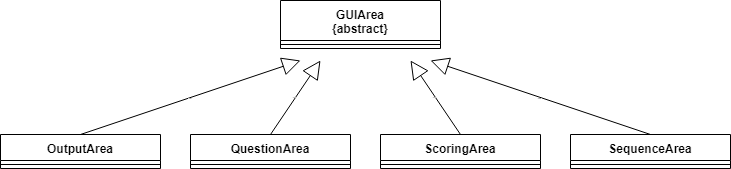
\includegraphics[page=1, width=0.7\paperwidth, trim=0 0 0 0, clip]{fig/GUIArea.png} 
            \caption{Übersicht über die GUIAreas}
            \label{fig:sql-run}
        \end{center}
    \end{figure}

Die Idee hinter der Struktur dieser Klassen basiert darauf, dass sich die GUI von Fragenplugins in \eigenname{ILIAS} in drei Szenen einteilt. Eine Szene beschreibt die GUI beim Anlegen und Bearbeiten einer Szene, eine Zweite beschreibt die Fragenvorschau, so wie die Anzeige der eigentlichen Frage in einem Test, und eine Dritte betrifft die Anzeige der Lösung.

Dabei besitzt \eigenname{assSQLQuestion} vier GUI Bereiche, die sich in jeder dieser Szenen wiederholen (s.Abbildung \ref{fig:gui-bereiche}). Einmal gibt es den Bereich der die Frage wiedergibt - die \eigenname{QuestionArea} (Blau). Als zweites gibt es den Bereich der die \eigenname{SQL}-Sequenzen enthält, genannt \eigenname{SequenceArea} (Orange). Dann gibt es den Bereich der die Ausgabe beinhaltet, die  \eigenname{OutputArea} (Grün). Und es gibt die \eigenname{ScoringArea}, welche die Metriken umschließt (Gelb). 

    \begin{figure}[H]
        \begin{center}
            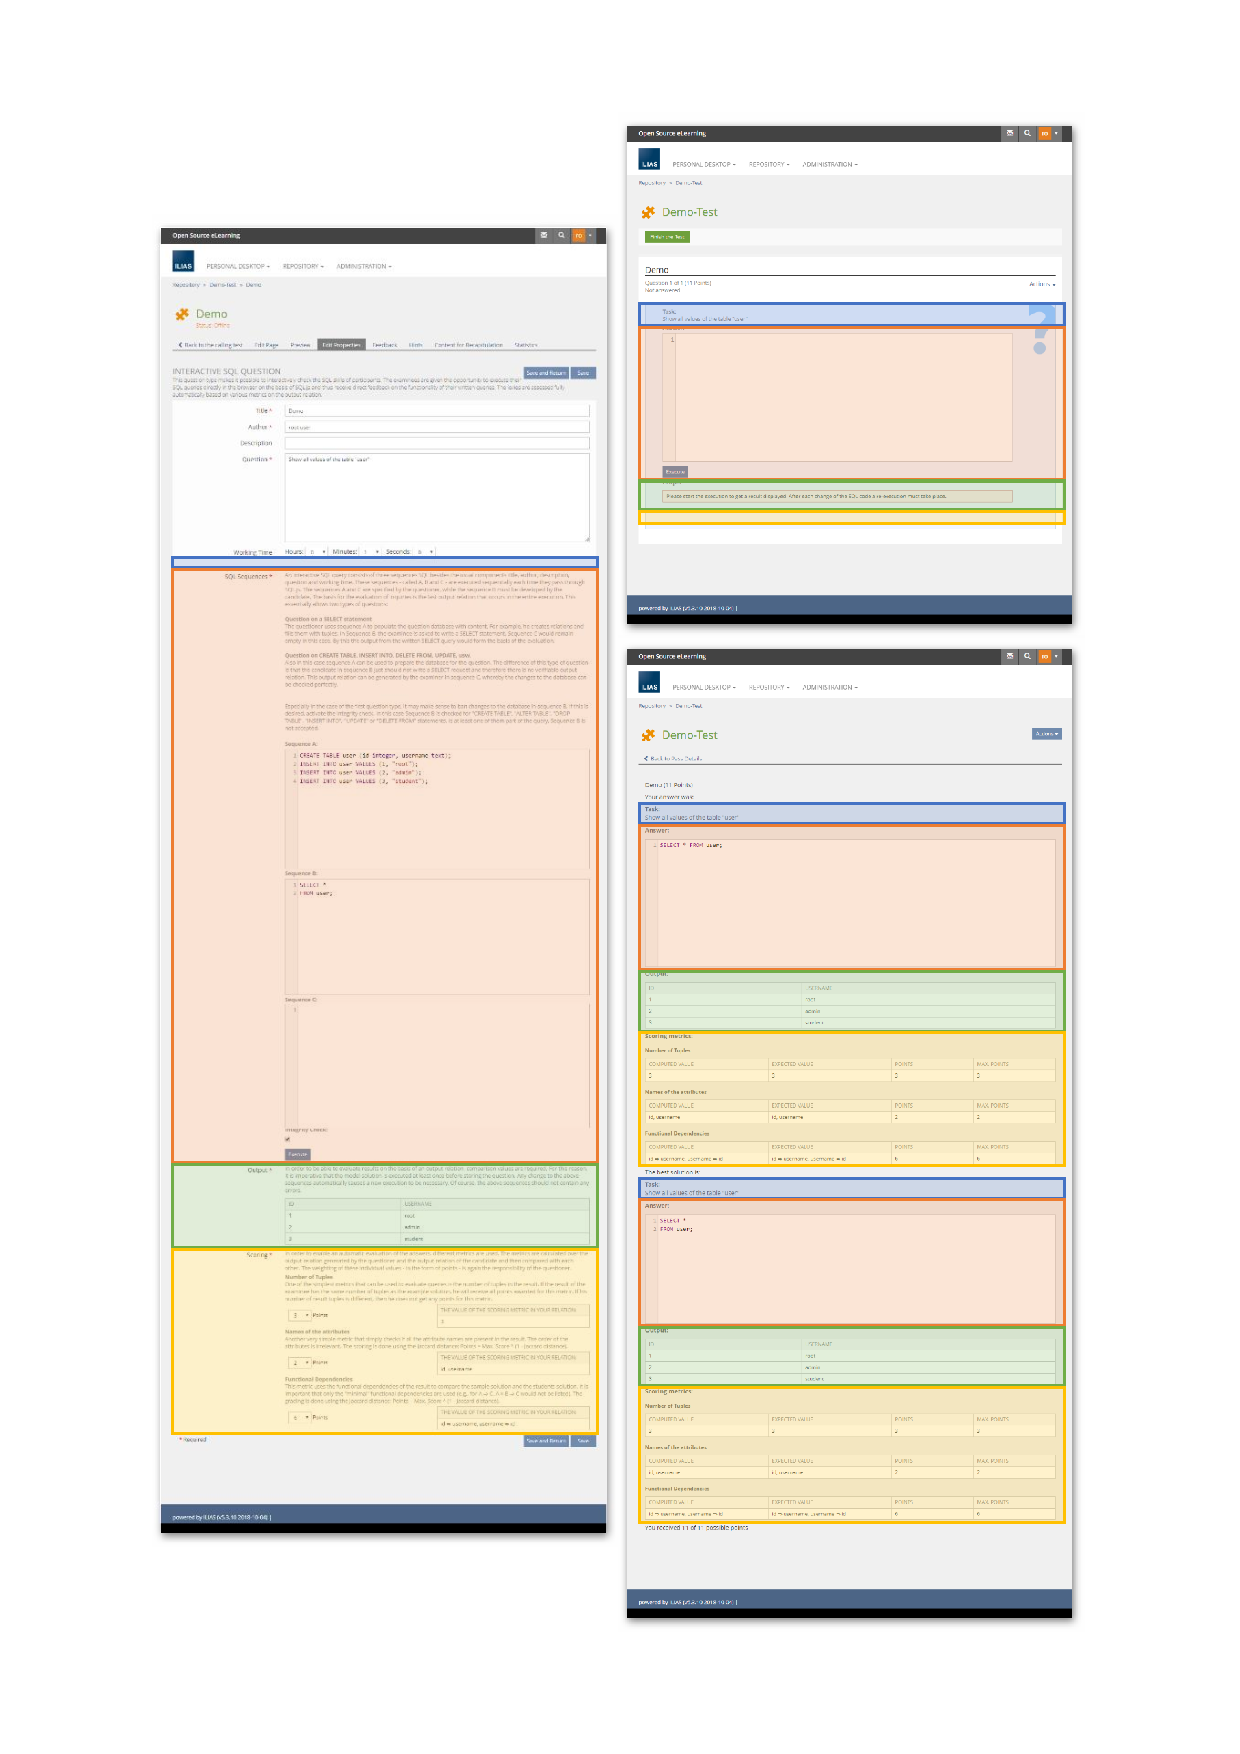
\includegraphics[page=1, width=0.7\paperwidth, trim=4 4 4 4, clip]{fig/GUIAreas.pdf} 
            \caption{GUI-Bereiche von assSQLQuestion}
            \label{fig:gui-bereiche}
        \end{center}
    \end{figure}
    
 




